\section[Deep Linguistic Structured Prediction and Independent
Factorization]{Deep Linguistic Structured Prediction and \\Independent
  Factorization}
\label{sec:background:deepsp}

Due to the power of representation learning, deep learning is widely
used to extract sophisticated representations for the inputs in
various NLP tasks. In this dissertation, instead of focusing on a single
task, we systematically study the representation learning challenges
for multiple tasks based on the independent factorization
assumption. In this section, We first introduce the recent advances
in deep structured prediction with respect to representational
formalism~(\autoref{ssec:bg:formalism}) and introduce the independent
factorization with factor graphs. Then we briefly summarize the
progress on representation learning for natural
language~(\autoref{ssec:bg:rep-learning}) and show why the independent
factorization is possible with the contextualized representations.
Finally, we also summarize the recent advances on
inference~(\autoref{ssec:bg:inference}) for linguistic structured prediction.

%In this dissertation, based on the independent factorization, we study the
%generic inductive biases for \textbf{different purposes more than the
%  accuracy on a single task or a single domain}. For example, by
%exploiting the known linguistic knowledge about anchoring, we study
%five \textit{cross-framework} meaning representation parsing with a
%lexical-anchoring parser and a . By defining two complementary
%dialogueue observers to sequentially predict the MISC code for both
%current and future utterance, our model emphasizes both
%\textit{accurate and real-time} assistance to a therapist. We propose
%to represent the output labels with natural language descriptions for
%\textit{zero-shot learning} on unseen labels~(\autoref{chap:sgd}). In our
%dissertation, we show that during the rapid progress of representation
%learning methods, our proposed inductive biases still can outperform
%the standard usage baselines.

\subsection{Formulations of Structural Interdependence}
\label{ssec:bg:formalism}

Structured prediction refers to machine learning models that learn a
target function to predict mulitple interrelated and dependent
outputs. For representing the target function, different formulations
exists. In this section, we mainly review the recent advances of
representations for modeling the structural interdependences.

\subsubsection{Graphical Models}
\label{sssec:bg:graphic-models}
A graphical model is a probabilistic model using a graph to express
the conditional dependence structure between random
variables. Generally, probabilistic graphical models use a graph-based
representation as the foundation for encoding a distribution over a
multidimensional space, which represents a set of independences that
hold in the specific distribution. Two branches of graphical
representations of distributions are commonly used, namely, Bayesian
networks and Markov random fields. Both families encompass the
properties of factorization and independence, but they differ in the
set of independences they can encode and the factorization of the
distribution that they induce.

\subsubsection{Constrained Conditional Models}
\label{sssec:bg:ccm}
Besides the graphical models to declaratively represent the structural
interdependence, constrained conditional
models~\citep[CCM,][]{chang2012structured} are for the same
goals. More specifically, CCM emphasizes augmenting the learning of
conditional models with declarative constraints. It aims to support
constrained decisions in an expressive output space while maintaining
modularity and tractability of training and inference. These
constraints can express either hard restrictions, completely
prohibiting some assignments, or soft limits, penalizing unlikely
assignments. One popular formalism to represent the constraints is to
use an integer linear programming~(ILP), which has been widely used to
constrain learning in many NLP tasks~\citep{roth2007global}. The
declarative linear objective functions, linear constraints, and the
availabilities of the off-the-shelf solvers make this formalism very
easy to use.

\subsubsection{Declarative Constraints in Deep Learning}
\label{sssec:bg:def-constraints}
Recently, to inject known hand-crafted constraints between discrete
variable assignments in the deep neural networks, one fundamental
challange is how to represent the constraints in end-to-end
differentiable ways~\citep{bach2017hinge}. For example,
\citet{li2019augmenting} propose to use differentiable fuzzy logic
operators to augment the neural networks with boolean
logic. \citet{pacheco2021modeling} introduce a declarative Deep
Relational Learning framework~(\DRAIL) integrating neural
representation learners with probabilistic logic. Besides representing
the constraints as logic forms, much recent work also studies
representing constraints with discrete latent variable models, such as
StructVAE for latent tree-structured
variables~\citep{yin2018structvae, corro2019learning}. Our work on
latent alignment models also falls into this category.

\subsubsection{Learning Constraints in Deep Learning}
\label{sssec:bg:learning-constraints}
Besides injecting declarative constraints, recent research also learn
the constraints in end-to-end
ways. \citet[SPEN,][]{belanger2016structured} define energy functions
that can learn the arbitrary dependencies among parts of structured
outputs by relaxing the whole structured outputs into continuous
vectors, Following this, inference network~\citep{tu2018learning} was
proposed to learn the constrained network for inference, which
approximates the cost-augmented inference during training and then
fine-tuning for test-time inference.

\subsubsection{Independent Factorization}
\label{sssec:bg:ind-factorization}
In this dissertation, we mainly use the undirected Markov random fileds to
represent our independent factorization assumptions. As shown
in~\autoref{fig:bg:graphical-model}, each circle represents a
variable, while each rectangle indicates a factor between the input
sentence variable $x$ and each decomposed segments of output
structures $y$. The difference between the left and right figure is in
the alignment variable $a$ in the center. In the left figure, the
shaded circle $a$ means the alignment is explicitly observed after the
decomposition. In the right figure, the alignment variable $a$ is not
observed.

\begin{figure}[!tbp]
\begin{center}
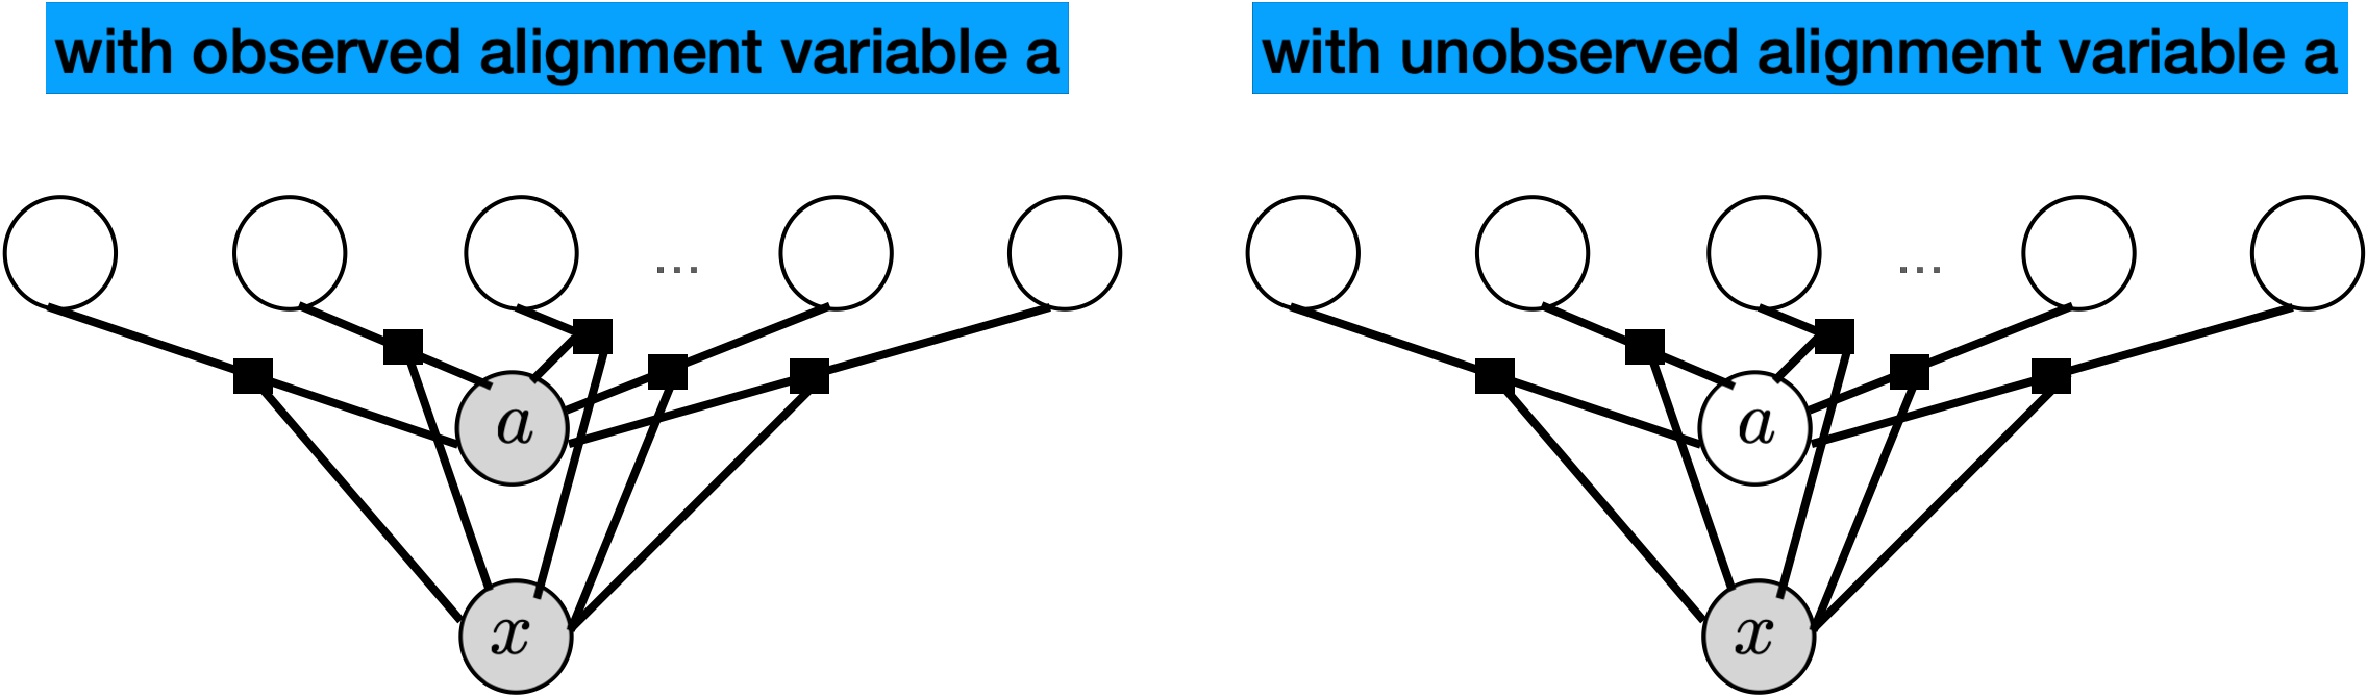
\includegraphics[width=0.90\textwidth]{graphical-models.pdf}
\end{center}
\caption{\label{fig:bg:graphical-model}The factor representation for
  the independent factorization used in our dissertation.}
\end{figure}

As discuessed in \autoref{ssec:intro:bias-dsp}, to apply independent
factorization for each task, we need to resolve three main challenges
to formulate the above factor graph as
$E(x, y) = \sum_{c \in C}E(x, a(y_{c}), y_{c})$, including
\begin{inparaenum}[(1)]
\item \textbf{Output Decomposition:}~Decomposing the output $y$ into a set of independent parts
  $y_{c}$.
\item \textbf{Input Decomposition and Alignments Discovery:}~Decomposing $x$ and derive the aligned input $x_{a_{y_{c}}}$ at
  the index $a_{y_{c}}$.
\item \textbf{Factor Modeling:}~Modelling each $y_{c}$ and its
  relevant parts $x_{a_{y_{c}}}$ to compute the energy score
  $E(x, a(y_{c}), y_{c})$.
\end{inparaenum}

In the following subsection, we show that rapid progress in
contextualized representation learning can offer discriminative
features for modelling the relative parts of $x_{a_{y_{c}}}$, thus
make the challenge~(3)~(factor modeling) of independent factorization possible. Then we
provide the background knowledge about structures in NLP in
\autoref{sec:bg:symbolic}, and we briefly show that such prior
knowledge about anchoring and compositionality are the main source of
inductive biases that guide us to find the decomposition and alignment
in the challenge (1) and (2). We extend the detailed analysis about
independent factorization in each application chapter.

\subsection{Neural Representation Learning}
\label{ssec:bg:rep-learning}

Structured prediction requires the learning can capture both the
discriminative interactions between $x$ and $y$ and also allow
efficient combinatorial optimization over $y$. Ideally, we hope neural
representation learning can handle all of this.

The key challenge of trying to apply analytical and computational
methods to text data are how to represent the text in a way that is
amenable to operations such as similarity, composition, etc. Besides
the early day one-hot representation and TF-IDF
extensions~\citep{jones1972statistical}, word embedding and neural
contextualized representation are widely used in modern deep learning
based models. In this section, we review the recent advances from
static word embedding based methods to attention-based dynamic
features selection and contextualized representation. Finally, we also
introduced the rapid progress in language encoding architectures, from
recurrent neural networks to transformer, and the corresponding
pretrained language models ELMo~\citep{Peters:2018},
BERT~\citep{devlin2019bert}, GPT3~\cite{brown2020language}, etc.

\subsubsection{Static Word Embedding}
\label{sssec:bg:static-embedding}
Word embeddings are commonly categorized into two
types~\citep{Baroni:2014,pennington2014glove,li2015generative},
depending upon the strategies used to induce them:
\begin{inparaenum}[(1)]
\item Prediction-based models, via local data in sentence~(a word'
  context).
\item Count-based models, via the global corpus-wide statistics~(such
  as word counts, co-occurrece).
\end{inparaenum}

Skip-gram with negative sampling~\cite[SGNS,][]{mikolov13w2v} and
GloVe~\cite{pennington2014glove} are among the best-known models for
the two types, respectively. However, they create a single fixed
representation for each word, a notable problem with the static word
embeddings are that all senses of a polysemous word must share a single
vector.

\subsubsection{Contextualized Representation}
\label{sssec:bg:contextualizing}
To resolve the above issue of static word embedding, sequence
encoders, such as LSTM~\citep{hochreiter97lstm},
Transformer~\citep{NIPS2017_7181}, can be used as contextualizing
models to encode the whole context and produce a \kw{contexualized
  representation} for each word, phrase or the whole sentence. In this
way, the contextualized representation dynamically depends on the
entire sentence. Furthermore, based on the neural sequence encoding
architectures, pretraining language models with a large amount of text
can create a more powerful contextualized
representations~\citep{ethayarajh2019contextual}. ELMo~\cite{Peters:2018}
creates contextualized representations of each token by concatenating
the internal states of a 2-layer BiLSTM trained on a bidirectional
language modeling task. In contrast, BERT~\citep{devlin2019bert} and
GPT-2~\citep{radford2018improving} are bidirectional and
unidirectional transformer-based language models,
respectively. \citet{peters2019tune} shows that ELMo contextualized
representation is more suitable to be used as a fixed word embedding,
as also shown in our dissertation on lexical and phrasal anchoring
based parsing~(\autoref{chap:lexical-phrasal}) and sentenctial
anchoring based MISC code prediction~(\autoref{chap:snt}). While for
BERT and GPT-2, finetuning them on downstream task will lead to better
performance, which also inspired us on exploiting natural language
description to understand each output components~(such as intent, slot
labels)~in task-oriented dialogue~(\autoref{chap:sgd}).  One
assumption behind the independent factorization is that local models
with rich features may perform competitively or better than global
models also exists in the pre deep-learning era. Before the rising of deep
learning in 2012, the well known MEMM-based Stanford pos tagger is the
state-of-art model at that time. Instead of using a single normalized,
global CRF model for the sequence modeling, richer features seem
diminish the label biases problems in the
MEMM~\citep{toutanvoa2000enriching,toutanova2003feature}. However, the
rich global features required heavy engineering in ten years ago.
Recently, according to the NLP-Progress
website,~\footnote{\url{http://nlpprogress.com/english/named_entity_recognition.html}
  visited on July 19, 2022}~which tracks the state-of-art models for
each task, we found that the state-of-art models for many sequences
tagging tasks~(such as named entity recognization, part-of-speech
tagging) are attention-based models without any CRF layer. In this
dissertation, the contextualized representation learned from deep
learning is the key to our independent factorization, which helps our
decomposed factor models to make local decisions with a set of
discriminative and global features, without any heavy feature
engineering. Furthermore, large pretrained language model also offers
great power to use natural language in our modeling, such as
prompt-based models~\citep{shin2020autoprompt,liu2021pre}.

\subsection{Inference}
\label{ssec:bg:inference}

Learning with structured data typically involves searching or summing
over a set with an exponential number of structured elements, for
example, the set of all parse trees for a given sentence. In the deep
learning community, it is common to fit models by computing point
estimates, such as the MLE or MAP estimate. Such MAP inference
approaches seem particularly appealing since they are computationally
fairly cheap and can use the before reducing overfitting. In this
way, the neural models only learn a single set of parameters. However,
the point estimation does not capture the associated
uncertainties~\citep{murphy2022probabilistic,wilson2020bayesian}.
Hence, we care about both MAP
and marginal inference in structured prediction research.

\subsubsection{MAP Inference}
\label{sssec:bg:map-inference}
Various exact inference methods are proposed
for MAP inference in NLP tasks. Exact inference methods include
dynamic programming based methods~(such as
viterbi~\citep{viterbi1967error} for hidden markov models, CKY for
context-tree
grammars~\citep{kasami1966efficient,younger1967recognition,cocke1969programming}
, Max Spanning Arborescence for spanning
tree~\citep{chu1965shortest,edmonds1967optimum}, and so on), and
Integer Linear
Programming~\citep{roth2005integer,roth2007global,berant2014modeling}. On the other side, approximate inference methods include various
sampling methods~\citep{finkel2005incorporating,singh2012monte},
search-based
methods~\citep{daume2009search,ross2011reduction,chang2015learning},
and Linear Programming
Relaxations~\citep{rush2012tutorial,werner2014power}.

\subsubsection{Marginal Inference}
\label{sssec:bg:marginal-inference}
Integration is at the heart of marginal inference, whereas
differentiation is at the heart of optimization. Corresponding to the
each of the above exact MAP inference algorithms, various methods are
proposed for marginal inference. They compute marginal probabilities
and partition functions which are central to many methods, such as
EM~\citep{baker1979trainable,weizenbaum1966eliza}, constrative
estimation~\citep{smith2005contrastive}, Conditional Random
Field~\citep[CRF,][]{lafferty01crf}, max-margin training over all
candidate targets~\citep{koller2004max}. For linguistic structured
prediction, exact marginal inference methods include forward-backward
algorithm for HMM~\citep{binder1997space},
Inside-outside~\citep{baker1979trainable}, Matrix-Tree Theorem for
nonprojective dependency
structures~\citep{koo-etal-2007-structured,liu2018learning}.

In this dissertation, we use variational inference to marginalize out the
latent alignment variable
in~\autoref{ssec:lex-phr:latent-alignment}. While for the other parts
of this dissertation, the assumption of independent factorization simplified
the inference into either greedy~(\autoref{chap:snt} and
\autoref{chap:sgd}) or dynamic programming based exact MAP
inference~(such as the dynamic programming parsing the dependency and
constituency structures in~\autoref{ssec:lex-phr:two-stage} and
~\autoref{sec:lex-phr:cky-based}, respectively)

%%% Local Variables:
%%% mode: latex
%%% TeX-master: "../../dissertation-main.ltx"
%%% End:
